\newcommand{\associatedObj}{associated\_obj}

 \begin{figure}
 	\centering
 	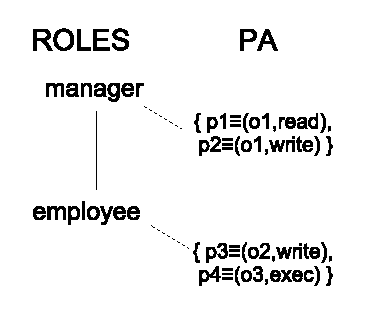
\includegraphics[width=.3\textwidth]{ABAC16/rbac-labac-example}
 	\caption{An example of roles and permission-role assignments in RBAC.}
 	\label{fig:rbac-labac-example}
 \end{figure}
 \begin{figure*}
 	\centering
 	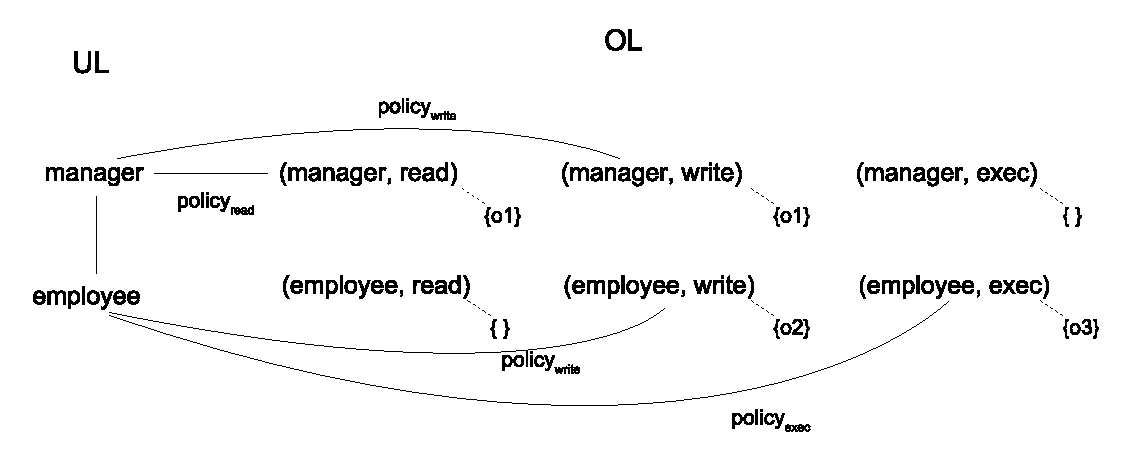
\includegraphics[width=.8\textwidth]{ABAC16/rbac-labac-configuration-explained}
 	\caption{An instance of RBAC (from Figure \ref{fig:rbac-labac-example}) configured in \eapABAC{}.}
 	\label{fig:rbac-labac-configuration-explained}
 \end{figure*}


 
%\begin{table}[]
\centering
\caption{Authorization policies in \hlabac{}  illustrating roles  in Figure \ref{fig:rbac-labac-example}}
\label{tab:rbac-labac-example-table}
\begin{tabular}{|l|l|l|l|}
	\hline
UL  & OL                                                                   & oLabel(o)                                                                          & Policy                                                                                                                                               \\
\hline
mng & \begin{tabular}[c]{@{}l@{}}\{mng\_read,\\ mng\_write\}\end{tabular}  & \begin{tabular}[c]{@{}l@{}}oLabel(o1)=\\ \{mng\_read, \\ mng\_write\}\end{tabular} & \begin{tabular}[c]{@{}l@{}} $p_{read} \equiv$ \\$\{(mng, mng\_read) \}$,\\ $p_{write} \equiv$ \\ $\{(mng, mng\_write)$,\}\end{tabular} \\ 
\hline
emp & \begin{tabular}[c]{@{}l@{}}\{emp\_write, \\ emp\_exec\}\end{tabular} & \begin{tabular}[c]{@{}l@{}}oLabel(o2)=\\ \{emp\_write, \\ emp\_exec\}\end{tabular} & \begin{tabular}[c]{@{}l@{}}$p_{read} \equiv$ \\ $\{(emp, emp\_write)\}$,\\ $p_{exec} \equiv $ \\ $\{(emp,  emp\_exec)\}$\end{tabular}       \\
\hline                                               
\end{tabular}
\end{table}



\newcommand{\sessionRoles}{session\_roles}
\begin{table}
	\centering
	\caption{ $RBAC_1$ in \hlabac} %\vspace*{3pt}
	\label{tab:rbac-in-labac-table}
	\begin{tabular}{|l|}						
		\hline					
		\multicolumn{1}{|c|}{\underline{\textit{I. $RBAC_1$ components }}}\\				 
		 -  \textit{USERS, OBS, OPS, SESSIONS, ROLES} and \textit{RH} \\ \hfill (users,  objects, operations, sessions, roles \\ \hfill and role hierarchy resp.) \\
		 -  $\textit{PRMS} = {(\textit{OBS} \times \textit{OPS})}$, the set of permissions  \\		 
		 -  $\textit{UA} \subseteq \textit{USERS} \times \textit{ROLES}$.  \\
		 - $\textit{PA} \subseteq \textit{PRMS} \times \textit{ROLES}$. \\	
		 - $session\_user: \textit{SESSIONS} \to USERS$ \\
		 %- $\sessionRoles: \textit{SESSIONS} \to 2^{\textit{ROLES}}$ ; $\sessionRoles(s) \subseteq$ \\ \hfill  $  \{r | (\exists r' \succeq r)[session\_user(s),r') \in \textit{UA}]\}$\\
		  - $\sessionRoles: \textit{SESSIONS} \to 2^{\textit{ROLES}}$ and \\ \hfill $\sessionRoles(s) \subseteq  \{r | (\exists r' \succeq r)[session\_user(s),r') \in \textit{UA}]\}$\\
		\\\multicolumn{1}{|c|}{\underline{\textit{II. Construction in \hlabac}}} \\
		 	-  $U = \textit{USERS}, O = \textit{OBS}, A = \textit{OPS}, S=\textit{SESSIONS} $ \\ 
		 	- \textit{UL=ROLES, ULH=RH}\\		  
		 	- $ OL = \textit{ROLES} \times \textit{OPS}$, $\textit{OLH}= \{ \}$\\
		 	-  $\uLabel(u) = \{ r | (u,r) \in UA \}$ \\
		 	
		 	-  $ \oLabel(o) = \{ (r,op) | ((o,op),r) \in PA \}$\\
		 	- $\creator(s) = session\_user(s)$, for $s \in S$	\\
		 	- $\sessionLabels(s) = \sessionRoles(s)$, for $s \in S$\\
		 	-  $\policy_{op_i} = \{ (r, (r',op_i) ) |  ((o,op_i),r')  \in PA \land r' = r  \} $ \\
		 	%- $\impliedPolicy_{op_i}$ and $\request()$ functions  are \\ \hfill unchanged from Table \ref{tab:labac-definition}	\\	
		 	
%		 	 \\ \multicolumn{1}{|c|}{\underline{\textit{III. Condition on session functions}}} \\
%		 	 - $\createSession(u,s,values)$: \\ \hfil $u \in U \land s \not \in S \land values \subseteq \uLabel(u)$\\
%		 	 - $\deleteSession(u,s)$: \\ \hfil $u \in U \land s \in S \land \creator(s)=u$\\
%		 	 - $\assignValues(u,s,values)$: \\ \hfil $u \in U \land s \in S \land \creator(s)=u \land values \subseteq \uLabel(u)  $ \\ 
%		 	 - $\removeValues(u,s,value)$: \\ \hfil $u \in U \land s \in S \land \creator(s)=u \land value \subseteq \uLabel(u)$ \\
		 	
		 \hline	
	\end{tabular}	

	
\end{table}

 
%\subsection{RBAC in \hlabac} 
A definition of hierarchical RBAC ($RBAC_1$) is shown in Segment I of Table \ref{tab:rbac-in-labac-table}. In RBAC, permissions are assigned to roles and users receive permissions through their enrollment to roles. Roles are partially ordered. If a role, $r_i$ is senior to role, $r_j$ (otherwise told $r_i$ dominates $r_j$), $r_i$ inherits permissions from $r_j$ and $r_j$ inherits users from $r_i$. Thus role hierarchy serves dual purpose of inheriting users and permissions. Figure \ref{fig:rbac-labac-example} presents an example showing roles, role hierarchy and permission-role assignments in $RBAC_1$. 

In Segment II of Table \ref{tab:rbac-in-labac-table}, we show  construction of $RBAC_1$ in \hlabac. Minimalistically, we need \clabac{}, but we use \hlabac{} for convenience. 



Figure  \ref{fig:rbac-labac-configuration-explained} shows an instance of RBAC (given in Figure \ref{fig:rbac-labac-example}) configured in LaBAC. In the figure, user-label values and its hierarchy directly correspond to roles and role hierarchy of Figure \ref{fig:rbac-labac-example}. On the other hand, object-label values correspond to Cartesian Product of $ROLES$ and $OPS$.   For example, for roles \{$manager, employee$\} and operations $\{read, write, exec\}$ of Figure \ref{fig:rbac-labac-example}, six different object-label values have been defined.  For an object-label value $(r,op)$, we assign it to the object $o$  if $(o,op)$ is a permission assigned to role $r$. For example, object $o1$ is assigned to label $(manager,read)$ because $(o1,read)$ is  a permission of role $manager$ (see Figure \ref{fig:rbac-labac-example}). Having assigned object-label and user-label values, for each $r \in ROLES$,  we specify authorization policy $\Policy_{op} \equiv \{(r,(r,op))\}$ so that object labeled with $(r,op)$ are accessed by users labeled with role $r$ for operation $op$. For example, for role, $manager$ in Figure \ref{fig:rbac-labac-example}, we create $\policy_{read} \equiv \{(manager, (manager,read))\}$ and $\policy_{write} \equiv \{(manager, (manager,write))\}$. We do not create  policy $\policy_{exec} \equiv \{(manager, (manager, exec))\}$ because there is no permission defined with operation $exec$ in role $manager$. Table \ref{tab:rbac-in-labac-table} formally shows the configuration of $RBAC_1$ in LaBAC. 




\begin{table} 
	\centering
 \caption{Quantifying \eapABAC{} for simulating RBAC}
 \label{tab:rbac-labac-quantification}
 
 	\begin{tabular}{|l|}
 		\hline	                                                                                                           	
 		
 	$|UL| = |ROLES|$\\ 
 	$|OL| = |ROLES| \times |OPS|$\\
 	$|\Policy| = |OPS|$\\
 		\hline
 	\end{tabular}  
\end{table}
 
 

 
 Finally, Table \ref{tab:rbac-labac-quantification} presents number of user-label values, object-label values and authorization policies required to configure $RBAC_1$.  
 


 

